
%% bare_conf.tex
%% V1.3
%% 2007/01/11
%% by Michael Shell
%% See:
%% http://www.michaelshell.org/
%% for current contact information.
%%
%% This is a skeleton file demonstrating the use of IEEEtran.cls
%% (requires IEEEtran.cls version 1.7 or later) with an IEEE conference paper.
%%
%% Support sites:
%% http://www.michaelshell.org/tex/ieeetran/
%% http://www.ctan.org/tex-archive/macros/latex/contrib/IEEEtran/
%% and
%% http://www.ieee.org/

%%*************************************************************************
%% Legal Notice:
%% This code is offered as-is without any warranty either expressed or
%% implied; without even the implied warranty of MERCHANTABILITY or
%% FITNESS FOR A PARTICULAR PURPOSE! 
%% User assumes all risk.
%% In no event shall IEEE or any contributor to this code be liable for
%% any damages or losses, including, but not limited to, incidental,
%% consequential, or any other damages, resulting from the use or misuse
%% of any information contained here.
%%
%% All comments are the opinions of their respective authors and are not
%% necessarily endorsed by the IEEE.
%%
%% This work is distributed under the LaTeX Project Public License (LPPL)
%% ( http://www.latex-project.org/ ) version 1.3, and may be freely used,
%% distributed and modified. A copy of the LPPL, version 1.3, is included
%% in the base LaTeX documentation of all distributions of LaTeX released
%% 2003/12/01 or later.
%% Retain all contribution notices and credits.
%% ** Modified files should be clearly indicated as such, including  **
%% ** renaming them and changing author support contact information. **
%%
%% File list of work: IEEEtran.cls, IEEEtran_HOWTO.pdf, bare_adv.tex,
%%                    bare_conf.tex, bare_jrnl.tex, bare_jrnl_compsoc.tex
%%*************************************************************************

% *** Authors should verify (and, if needed, correct) their LaTeX system  ***
% *** with the testflow diagnostic prior to trusting their LaTeX platform ***
% *** with production work. IEEE's font choices can trigger bugs that do  ***
% *** not appear when using other class files.                            ***
% The testflow support page is at:
% http://www.michaelshell.org/tex/testflow/



% Note that the a4paper option is mainly intended so that authors in
% countries using A4 can easily print to A4 and see how their papers will
% look in print - the typesetting of the document will not typically be
% affected with changes in paper size (but the bottom and side margins will).
% Use the testflow package mentioned above to verify correct handling of
% both paper sizes by the user's LaTeX system.
%
% Also note that the "draftcls" or "draftclsnofoot", not "draft", option
% should be used if it is desired that the figures are to be displayed in
% draft mode.
%
\documentclass[conference]{IEEEtran}

\IEEEoverridecommandlockouts
% Add the compsoc option for Computer Society conferences.
%
% If IEEEtran.cls has not been installed into the LaTeX system files,
% manually specify the path to it like:
% \documentclass[conference]{../sty/IEEEtran}





% Some very useful LaTeX packages include:
% (uncomment the ones you want to load)


% *** MISC UTILITY PACKAGES ***
%
%\usepackage{ifpdf}
% Heiko Oberdiek's ifpdf.sty is very useful if you need conditional
% compilation based on whether the output is pdf or dvi.
% usage:
% \ifpdf
%   % pdf code
% \else
%   % dvi code
% \fi
% The latest version of ifpdf.sty can be obtained from:
% http://www.ctan.org/tex-archive/macros/latex/contrib/oberdiek/
% Also, note that IEEEtran.cls V1.7 and later provides a builtin
% \ifCLASSINFOpdf conditional that works the same way.
% When switching from latex to pdflatex and vice-versa, the compiler may
% have to be run twice to clear warning/error messages.






% *** CITATION PACKAGES ***
%
%\usepackage{cite}
% cite.sty was written by Donald Arseneau
% V1.6 and later of IEEEtran pre-defines the format of the cite.sty package
% \cite{} output to follow that of IEEE. Loading the cite package will
% result in citation numbers being automatically sorted and properly
% "compressed/ranged". e.g., [1], [9], [2], [7], [5], [6] without using
% cite.sty will become [1], [2], [5]--[7], [9] using cite.sty. cite.sty's
% \cite will automatically add leading space, if needed. Use cite.sty's
% noadjust option (cite.sty V3.8 and later) if you want to turn this off.
% cite.sty is already installed on most LaTeX systems. Be sure and use
% version 4.0 (2003-05-27) and later if using hyperref.sty. cite.sty does
% not currently provide for hyperlinked citations.
% The latest version can be obtained at:
% http://www.ctan.org/tex-archive/macros/latex/contrib/cite/
% The documentation is contained in the cite.sty file itself.






% *** GRAPHICS RELATED PACKAGES ***
%
\ifCLASSINFOpdf
  % \usepackage[pdftex]{graphicx}
  % declare the path(s) where your graphic files are
  % \graphicspath{{../pdf/}{../jpeg/}}
  % and their extensions so you won't have to specify these with
  % every instance of \includegraphics
  % \DeclareGraphicsExtensions{.pdf,.jpeg,.png}
\else
  % or other class option (dvipsone, dvipdf, if not using dvips). graphicx
  % will default to the driver specified in the system graphics.cfg if no
  % driver is specified.
  % \usepackage[dvips]{graphicx}
  % declare the path(s) where your graphic files are
  % \graphicspath{{../eps/}}
  % and their extensions so you won't have to specify these with
  % every instance of \includegraphics
  % \DeclareGraphicsExtensions{.eps}
\fi
% graphicx was written by David Carlisle and Sebastian Rahtz. It is
% required if you want graphics, photos, etc. graphicx.sty is already
% installed on most LaTeX systems. The latest version and documentation can
% be obtained at: 
% http://www.ctan.org/tex-archive/macros/latex/required/graphics/
% Another good source of documentation is "Using Imported Graphics in
% LaTeX2e" by Keith Reckdahl which can be found as epslatex.ps or
% epslatex.pdf at: http://www.ctan.org/tex-archive/info/
%
% latex, and pdflatex in dvi mode, support graphics in encapsulated
% postscript (.eps) format. pdflatex in pdf mode supports graphics
% in .pdf, .jpeg, .png and .mps (metapost) formats. Users should ensure
% that all non-photo figures use a vector format (.eps, .pdf, .mps) and
% not a bitmapped formats (.jpeg, .png). IEEE frowns on bitmapped formats
% which can result in "jaggedy"/blurry rendering of lines and letters as
% well as large increases in file sizes.
%
% You can find documentation about the pdfTeX application at:
% http://www.tug.org/applications/pdftex





% *** MATH PACKAGES ***
%
%\usepackage[cmex10]{amsmath}
% A popular package from the American Mathematical Society that provides
% many useful and powerful commands for dealing with mathematics. If using
% it, be sure to load this package with the cmex10 option to ensure that
% only type 1 fonts will utilized at all point sizes. Without this option,
% it is possible that some math symbols, particularly those within
% footnotes, will be rendered in bitmap form which will result in a
% document that can not be IEEE Xplore compliant!
%
% Also, note that the amsmath package sets \interdisplaylinepenalty to 10000
% thus preventing page breaks from occurring within multiline equations. Use:
%\interdisplaylinepenalty=2500
% after loading amsmath to restore such page breaks as IEEEtran.cls normally
% does. amsmath.sty is already installed on most LaTeX systems. The latest
% version and documentation can be obtained at:
% http://www.ctan.org/tex-archive/macros/latex/required/amslatex/math/





% *** SPECIALIZED LIST PACKAGES ***
%
%\usepackage{algorithmic}
% algorithmic.sty was written by Peter Williams and Rogerio Brito.
% This package provides an algorithmic environment fo describing algorithms.
% You can use the algorithmic environment in-text or within a figure
% environment to provide for a floating algorithm. Do NOT use the algorithm
% floating environment provided by algorithm.sty (by the same authors) or
% algorithm2e.sty (by Christophe Fiorio) as IEEE does not use dedicated
% algorithm float types and packages that provide these will not provide
% correct IEEE style captions. The latest version and documentation of
% algorithmic.sty can be obtained at:
% http://www.ctan.org/tex-archive/macros/latex/contrib/algorithms/
% There is also a support site at:
% http://algorithms.berlios.de/index.html
% Also of interest may be the (relatively newer and more customizable)
% algorithmicx.sty package by Szasz Janos:
% http://www.ctan.org/tex-archive/macros/latex/contrib/algorithmicx/




% *** ALIGNMENT PACKAGES ***
%
%\usepackage{array}
% Frank Mittelbach's and David Carlisle's array.sty patches and improves
% the standard LaTeX2e array and tabular environments to provide better
% appearance and additional user controls. As the default LaTeX2e table
% generation code is lacking to the point of almost being broken with
% respect to the quality of the end results, all users are strongly
% advised to use an enhanced (at the very least that provided by array.sty)
% set of table tools. array.sty is already installed on most systems. The
% latest version and documentation can be obtained at:
% http://www.ctan.org/tex-archive/macros/latex/required/tools/
\usepackage{amsmath}

%\usepackage{mdwmath}
%\usepackage{mdwtab}
% Also highly recommended is Mark Wooding's extremely powerful MDW tools,
% especially mdwmath.sty and mdwtab.sty which are used to format equations
% and tables, respectively. The MDWtools set is already installed on most
% LaTeX systems. The lastest version and documentation is available at:
% http://www.ctan.org/tex-archive/macros/latex/contrib/mdwtools/


% IEEEtran contains the IEEEeqnarray family of commands that can be used to
% generate multiline equations as well as matrices, tables, etc., of high
% quality.


%\usepackage{eqparbox}
% Also of notable interest is Scott Pakin's eqparbox package for creating
% (automatically sized) equal width boxes - aka "natural width parboxes".
% Available at:
% http://www.ctan.org/tex-archive/macros/latex/contrib/eqparbox/





% *** SUBFIGURE PACKAGES ***
%\usepackage[tight,footnotesize]{subfigure}
% subfigure.sty was written by Steven Douglas Cochran. This package makes it
% easy to put subfigures in your figures. e.g., "Figure 1a and 1b". For IEEE
% work, it is a good idea to load it with the tight package option to reduce
% the amount of white space around the subfigures. subfigure.sty is already
% installed on most LaTeX systems. The latest version and documentation can
% be obtained at:
% http://www.ctan.org/tex-archive/obsolete/macros/latex/contrib/subfigure/
% subfigure.sty has been superceeded by subfig.sty.



%\usepackage[caption=false]{caption}
%\usepackage[font=footnotesize]{subfig}
% subfig.sty, also written by Steven Douglas Cochran, is the modern
% replacement for subfigure.sty. However, subfig.sty requires and
% automatically loads Axel Sommerfeldt's caption.sty which will override
% IEEEtran.cls handling of captions and this will result in nonIEEE style
% figure/table captions. To prevent this problem, be sure and preload
% caption.sty with its "caption=false" package option. This is will preserve
% IEEEtran.cls handing of captions. Version 1.3 (2005/06/28) and later 
% (recommended due to many improvements over 1.2) of subfig.sty supports
% the caption=false option directly:
%\usepackage[caption=false,font=footnotesize]{subfig}
%
% The latest version and documentation can be obtained at:
% http://www.ctan.org/tex-archive/macros/latex/contrib/subfig/
% The latest version and documentation of caption.sty can be obtained at:
% http://www.ctan.org/tex-archive/macros/latex/contrib/caption/




% *** FLOAT PACKAGES ***
%
%\usepackage{fixltx2e}
% fixltx2e, the successor to the earlier fix2col.sty, was written by
% Frank Mittelbach and David Carlisle. This package corrects a few problems
% in the LaTeX2e kernel, the most notable of which is that in current
% LaTeX2e releases, the ordering of single and double column floats is not
% guaranteed to be preserved. Thus, an unpatched LaTeX2e can allow a
% single column figure to be placed prior to an earlier double column
% figure. The latest version and documentation can be found at:
% http://www.ctan.org/tex-archive/macros/latex/base/



%\usepackage{stfloats}
% stfloats.sty was written by Sigitas Tolusis. This package gives LaTeX2e
% the ability to do double column floats at the bottom of the page as well
% as the top. (e.g., "\begin{figure*}[!b]" is not normally possible in
% LaTeX2e). It also provides a command:
%\fnbelowfloat
% to enable the placement of footnotes below bottom floats (the standard
% LaTeX2e kernel puts them above bottom floats). This is an invasive package
% which rewrites many portions of the LaTeX2e float routines. It may not work
% with other packages that modify the LaTeX2e float routines. The latest
% version and documentation can be obtained at:
% http://www.ctan.org/tex-archive/macros/latex/contrib/sttools/
% Documentation is contained in the stfloats.sty comments as well as in the
% presfull.pdf file. Do not use the stfloats baselinefloat ability as IEEE
% does not allow \baselineskip to stretch. Authors submitting work to the
% IEEE should note that IEEE rarely uses double column equations and
% that authors should try to avoid such use. Do not be tempted to use the
% cuted.sty or midfloat.sty packages (also by Sigitas Tolusis) as IEEE does
% not format its papers in such ways.





% *** PDF, URL AND HYPERLINK PACKAGES ***
%
%\usepackage{url}
% url.sty was written by Donald Arseneau. It provides better support for
% handling and breaking URLs. url.sty is already installed on most LaTeX
% systems. The latest version can be obtained at:
% http://www.ctan.org/tex-archive/macros/latex/contrib/misc/
% Read the url.sty source comments for usage information. Basically,
% \url{my_url_here}.


\usepackage[utf8]{inputenc}
\usepackage{graphicx}
\usepackage[ngerman]{babel}

% *** Do not adjust lengths that control margins, column widths, etc. ***
% *** Do not use packages that alter fonts (such as pslatex).         ***
% There should be no need to do such things with IEEEtran.cls V1.6 and later.
% (Unless specifically asked to do so by the journal or conference you plan
% to submit to, of course. )


% correct bad hyphenation here
\hyphenation{op-tical net-works semi-conduc-tor}


\begin{document}

%
% paper title
% can use linebreaks \\ within to get better formatting as desired
\title{Neuartige Software-Defined Networking basierte Cloud zur Unterstützung des intelligenten Fahrzeugnetzwerks}
%

%Software Defined Networking for RSU Clouds in support of The Internet of Vehicles

% author names and affiliations
% use a multiple column layout for up to three different
% affiliations
\author{\IEEEauthorblockN{Christoph Wittmann}
\IEEEauthorblockA{Lehrstuhl für Kommunikationsnetze\\
Technische Universität München\\
Email: christoph.wittmann@tum.de}
%\and
%\IEEEauthorblockN{Your supervisor is NOT! an author of your paper!}
%\IEEEauthorblockA{Starfleet Academy\\
%San Francisco, California 96678-2391\\
%Telephone: (800) 555--1212\\
%Fax: (888) 555--1212}

\thanks{*This paper is a reinterpretation of the paper \emph{Mohammad A. Salahuddin, Ala Al-Fuqaha, Mohsen Guizani. ``Software Defined Networking for RSU Clouds in support of The Internet of Vehicles,'' Internet of Things Journal, IEEE, 2014, pp. 133-144}. It was presented on June 22, 2015 (Paper submission deadline) as a part of MSCE Seminar (MSCE course TUM), under the supervision of M. Sc. 
Christian Sieber (c.sieber@tum.de).}
}

% conference papers do not typically use \thanks and this command
% is locked out in conference mode. If really needed, such as for
% the acknowledgment of grants, issue a \IEEEoverridecommandlockouts
% after \documentclass

% for over three affiliations, or if they all won't fit within the width
% of the page, use this alternative format:
% 
%\author{\IEEEauthorblockN{Michael Shell\IEEEauthorrefmark{1},
%Homer Simpson\IEEEauthorrefmark{2},
%James Kirk\IEEEauthorrefmark{3}, 
%Montgomery Scott\IEEEauthorrefmark{3} and
%Eldon Tyrell\IEEEauthorrefmark{4}}
%\IEEEauthorblockA{\IEEEauthorrefmark{1}School of Electrical and Computer Engineering\\
%Georgia Institute of Technology,
%Atlanta, Georgia 30332--0250\\ Email: see http://www.michaelshell.org/contact.html}
%\IEEEauthorblockA{\IEEEauthorrefmark{2}Twentieth Century Fox, Springfield, USA\\
%Email: homer@thesimpsons.com}
%\IEEEauthorblockA{\IEEEauthorrefmark{3}Starfleet Academy, San Francisco, California 96678-2391\\
%Telephone: (800) 555--1212, Fax: (888) 555--1212}
%\IEEEauthorblockA{\IEEEauthorrefmark{4}Tyrell Inc., 123 Replicant Street, Los Angeles, California 90210--4321}}




% use for special paper notices
%\IEEEspecialpapernotice{(Invited Paper)}




% make the title area
\maketitle


\begin{abstract}
%\boldmath
Die Nachfrage nach Sicherheits- und Unterhaltungsdiensten im Straßenverkehr wächst unaufhörlich. Um diesen riesigen dynamischen Bedarf an Ressourcen zu bedienen, ist eine intelligente Lösung für das Fahrzeugnetzwerk vonnöten.
Einen großen Schritt zur Lösung dieser Problemstellung stellt die in diesem Paper vorgestellte neuartige Cloud Architektur dar. In dieser Architektur werden klassische Roadside Units (RSUs) und spezielle Software Defined Networking (SDN)-fähige RSUs zu einer RSU-Cloud zusammengefasst. Dank SDN lassen sich die gehosteten Dienste innerhalb der Cloud dynamisch verschieben, kopieren oder neu erzeugen, um sie der lokalen Nachfrage anzupassen. Das damit verbundene Problem des Ressourcen Managements in der Cloud wird als Mehrkriterielles Ganzzahliges Lineares Optimierungsproblem modelliert. Des Weitern wird ein heuristischer Ansatz präsentiert, um die Kosten einer Umkonfigurierung des Netzes zu minimieren. Die Heuristik wird zusätzlich durch den Einsatz von Bestärkendem Lernen hinsichtlich langfristiger Minimierung der Kosten verbessert.
Die Ergebnisse zeigen, dass die Heuristik verglichen mit einem naiven Ansatz bezüglich der Minimierung von Kosten und der Verzögerung im Netzwerk deutlich besser abschneidet. Auch die Verbesserung durch Bestärkendes Lernen macht sich längerfristig durch geringere Kosten bemerkbar.

\end{abstract}
% IEEEtran.cls defaults to using nonbold math in the Abstract.
% This preserves the distinction between vectors and scalars. However,
% if the conference you are submitting to favors bold math in the abstract,
% then you can use LaTeX's standard command \boldmath at the very start
% of the abstract to achieve this. Many IEEE journals/conferences frown on
% math in the abstract anyway.

% no keywords




% For peer review papers, you can put extra information on the cover
% page as needed:
% \ifCLASSOPTIONpeerreview
% \begin{center} \bfseries EDICS Category: 3-BBND \end{center}
% \fi
%
% For peerreview papers, this IEEEtran command inserts a page break and
% creates the second title. It will be ignored for other modes.
\IEEEpeerreviewmaketitle



\section{Einleitung}
% no \IEEEPARstart

Intelligente Transportsysteme bezeichnen ein Kommunikations-Framework für die Unterstützung des Reiseerlebnisses unabhängig von den Transportmitteln. Sie sind die Zukunft unserer Schienen, Straßen sowie Luft-und Wasserwege und ein großes aktuelles Forschungsgebiet. Durch die damit einhergehende Zusammenführung von Transport und Kommunikation wird sich ein großes Plus in Sachen Sicherheit, Effizienz und Ökologie versprochen. Dies soll unter anderem durch intelligente Ausbalancierung des Verkehrs zur Stauvermeidung oder durch die Warnung vor potentiellen Gefahrenstellen in Echtzeit erreicht werden. Gerade im Straßenverkehr werden jedoch von den Verkehrsteilnehmern auch immer mehr Dienste zur Unterhaltung, wie zum Beispiel Video Streaming, mobiles Internet und Internettelefonie nachgefragt. Diese Nachfrage an bandbreitenintensiven Anwendungen stellt große Anforderungen an ein Kommunikationsnetz. Hinzu kommt, dass sich der Bedarf an Ressourcen durch die naturgemäß hohe Mobilität der Verkehrsteilnehmer dynamisch ändert. Die Ressourcen müssen in der Regel bei einem Cloud Anbieter angemietet werden und verursachen Kosten für einen Dienstanbieter. Um diese Kosten zu minimieren, erfordert dies in der Praxis eine ständige bedarfsgerechte Umverteilung der Ressourcen und eine damit verbundene Neukonfiguration des Kommunikationsnetzes. Einen Lösungsansatz für diese Problemstellung hat Salahuddin et al. in einem Paper \cite{IEEEhowto:orig} mit dem 
Titel: \glqq Software Defined Networking for RSU Clouds in support of The Internet of Vehicles\grqq{} vorgestellt.
Dort wird eine neuartige Roadside Unit (RSU) Cloud Architektur beschrieben, die durch das Ausnutzen der Vorteile von Software Defined Networking (SDN) in hohem Maße flexibel konfigurierbar ist. Konkret bedeutet das, dass innerhalb der Cloud einzelne Dienste verschoben oder an einen anderen Ort kopiert werden, um der wechselnden lokalen Nachfrage gerecht zu werden. Solche Änderungen in der Cloud verursachen jedoch Kosten und können sich negativ auf die Netzwerk Performanz auswirken. Dies erfordert daher ein intelligentes Ressourcen Management, um diese notwendigen Änderungen zu minimieren. Dazu wird die Problemstellung als Mehrkriterielles Ganzzahliges Lineares Optimierungsproblem modelliert sowie eine Heuristik zur Problemlösung entwickelt.\\
Mein eigener Beitrag ist die Zusammenfassung der in \cite{IEEEhowto:orig} vorgestellten Cloud Architektur sowie des neuartigen Ressourcen Managements. Außerdem werde ich dieses Themengebiet durch relevante Hintergrundinformationen bezüglich SDN und durch die Darstellung anderer Cloud Architekturen ergänzen.\\
Dieses Paper gliedert sich wie folgt. Im Abschnitt II wird eine kurze Einführung in SDN und dessen Eigenschaften gegeben. In Abschnitt III finden sich eine Darstellung des Aufbaus einer RSU Cloud und deren Komponenten sowie die Anforderungen, die an eine RSU Cloud gestellt werden. Andere Cloud Architekturen und deren Vor- und Nachteile werden in Abschnitt IV erläutert. In Abschnitt V werden das Modell zum Ressourcen Management in der Cloud zusammengefasst. In Abschnitt VI werden die Ergebnisse der Simulationen präsentiert und mit anderen Ansätzen verglichen. Abschließend werde ich in Abschnitt VII die Ergebnisse zusammenfassen.



\section{Einführung in Software Defined Networking}

In diesem Kapitel wird ein Überblick über das Themengebiet SDN gegeben und die elementaren Eigenschaften des Konzepts dargelegt. Damit eine Technologie als SDN-fähig bezeichnet werden darf, müssen laut \cite{IEEEhowto:sdn} vier Prinzipien erfüllt sein, die ich im Folgenden kurz zusammenfassen möchte. Der zentrale Grundsatz in SDN ist die Trennung des Netzwerks in eine physikalische Datenebene und eine davon abstrahierte Kontrollebene. Das bedeutet, dass in einer SDN-fähigen Netzwerkkomponente eine von der Datenebene abgekoppelte, externe Instanz existieren muss. Diese Instanz wird Controller genannt und zeichnet sich dadurch aus, dass sie die Möglichkeit hat, das Weiterleitungsverhalten einer Netzwerkkomponente direkt zu bestimmen. In der Praxis besteht ein SDN daher aus Controllern und Switchen. In einem Switch sind nur noch die, von ihm auszuführenden Weiterleitungsvorschriften gespeichert, die dynamisch von einem Controller über die Kontrollebene aktualisiert werden können. Daraus ergibt sich zum Beispiel der Vorteil, dass Daten- und Kontrollebene im Design beziehungsweise in Untersuchungen und Analysen getrennt voneinander betrachtet werden können. \\
Ein weiteres Prinzip ist, dass ein derartiger Controller, obwohl er sich in einem SDN Netzwerk auf mehrere virtuelle oder physikalische Bestandteile verteilen kann, sich trotzdem logisch wie eine zentrale Einheit verhält, die über globales Wissen verfügt. Diese Eigenschaft bringt den Vorteil der schnelleren und effizienteren dynamischen Anpassung des Netzwerks.
Als dritter Grundsatz wird in \cite{IEEEhowto:sdn} die Offenheit der Schnittstellen genannt, worauf ich hier aber aus Relevanzgründen nicht näher eingehen möchte. Viel interessanter ist die Eigenschaft der Programmierbarkeit eines SDN Netzes. Dies wird durch die Entkopplung von Daten- und Kontrollebene ermöglicht und macht das Netzwerk extrem anpassbar an verschiedene Anwendungen. Laut \cite{IEEEhowto:sdn} lässt sich das Netzwerk dann als eine einzige programmierbare Einheit behandeln und nicht als eine Anhäufung von Geräten, die individuell konfiguriert werden müssen.\\
OpenFlow ist das am weitesten verbreitete Kommunikationsprotokoll, das in SDN eingesetzt wird. Es fungiert als Schnittstelle zwischen Datenebene und Kontrollebene, indem es direkten Zugriff auf Weiterleitungsverhalten eines Switches ermöglicht. Man spricht daher auch häufig von OpenFlow Kontrollern oder OpenFlow Switches. 


\section{Architektur der RSU Cloud}

Ein Fahrzeugnetzwerk (Vehicular Grid) besteht im Prinzip aus zwei Arten von Komponenten. Auf der einen Seite sind das Lokalisierungssysteme, Sensoren, Mikroprozessoren und Funkeinheiten, die an einem Fahrzeug montiert sind - sogenannte On-Board Units (OBUs) - und auf der anderen Seite  Sensoren und Mikrocontroller, die fest in die Straßen integriert sind, genannt Roadside Units (RSUs). Diese Komponenten vernetzt bilden ein sogenanntes Fahrzeug Ad hoc Netzwerk (VANET). Der neue Ansatz, der in diesem Paper diskutiert wird, ist die Zusammenfassung der RSUs zu einer RSU Cloud.\\
Da eine derartige Cloud demnach alle nachgefragten Sicherheits- sowie Unterhaltungsdienste bereitstellen können muss, werden hohe Anforderungen an sie gestellt. Eine RSU Cloud muss nicht nur verlässlich, sondern auch sehr leistungsstark hinsichtlich Datenrate und Latenz sein, um größtmögliche Sicherheit zu garantieren und somit die Akzeptanz in der Bevölkerung zu erlangen.\\

\begin{figure}[h!]
	\centering
	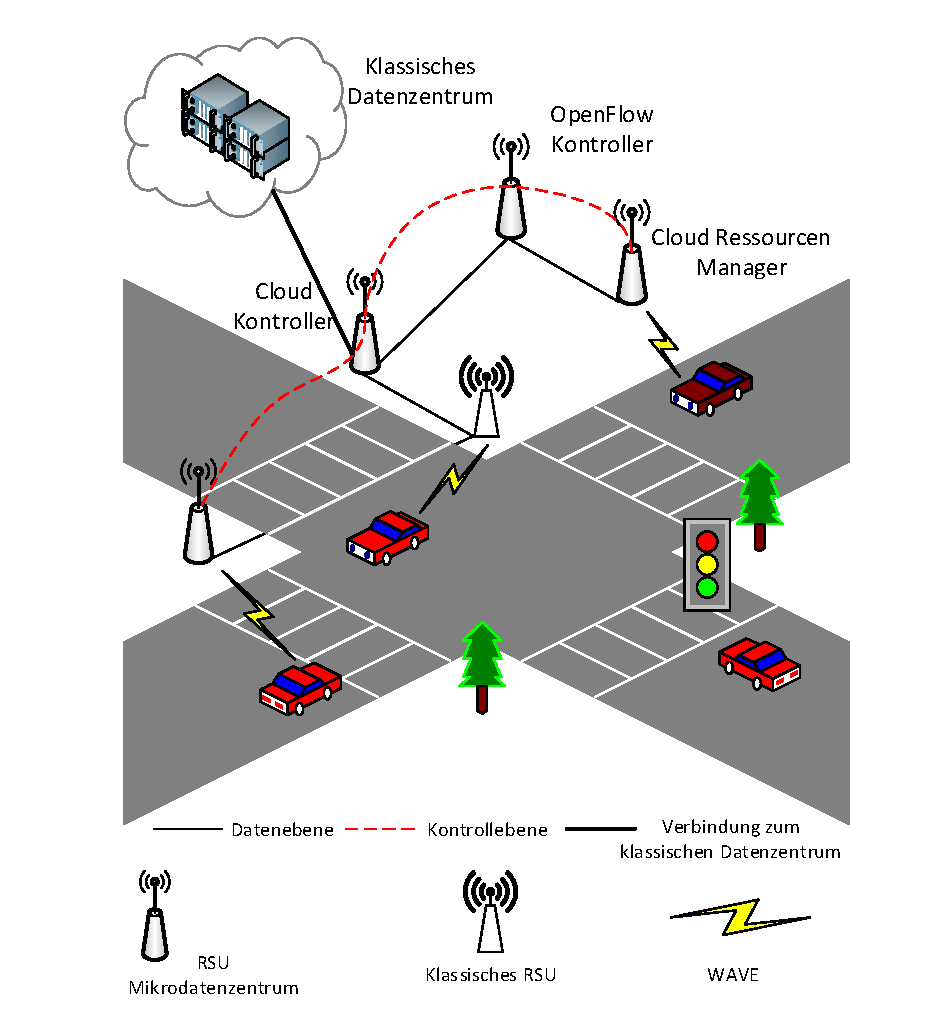
\includegraphics[trim=1.5cm 0 0 0.8cm, scale=0.66]{grafik/strasse.pdf}
	\caption{RSU Cloud Architektur}
	\label{img:grafik-dummy}
\end{figure}

Eine solche RSU Cloud besteht dabei neben gewöhnlichen RSUs zudem aus RSU Mikrodatenzentren. Ein Mikrodatenzentrum besteht aus einer kleinen Recheneinheit und einem OpenFlow Switch, sodass es in ein SDN Netzwerk eingebunden werden kann. Softwareseitig besteht ein Mikrodatenzentrum aus einem Betriebssystem und einem Hypervisor, der es mittels Virtualisierung ermöglicht, mehrere virtuelle Maschinen (VMs) dynamisch auf einem Host auszuführen. Auf einem solchen Mikrodatenzentrum sollen dann die Dienste gehostet werden, die von den Verkehrsteilnehmern nachgefragt werden. Dies hat den großen Vorteil, dass die Dienste sehr \glqq nah\grqq{} an den Konsumenten sind, was sich in einer höheren Verlässlichkeit und kürzeren Latenzzeiten bemerkbar macht. Die, zum Aufspannen einer Cloud in einem SDN Netzwerk, nötigen Softwarekomponenten wie ein OpenFlow Controller oder ein Cloud Kontroller sollen - wie in Abbildung \ref{img:grafik-dummy} zu sehen ist - ebenfalls in manchen Mikrodatenzentren ausgeführt werden. Eine weitere neue Komponente, die im Originalpaper vorgestellt wurde, ist der RSU Cloud Ressourcen Manager (CRM). Zudem ist auch der CRM in manchen Mikrodatenzentren integriert und soll Informationen über das Hosten von Diensten, die Verschiebung von Diensten oder das Ändern von Weiterleitungsvorschriften verbreiten, indem er mit OpenFlow und Cloud Kontrollern kommuniziert. Des Weiteren hat er die Aufgabe, die richtigen Entscheidungen bezüglich der optimalen Lage und Anzahl an gehosteten Diensten und den dazugehörigen Weiterleitungsvorschriften zu treffen. Entscheidend ist hierbei, dass die Anzahl an Verschiebungen von VMs möglichst gering gehalten wird, da sie zusätzlichen Netzwerkverkehr in Daten und Kontrollebene produzieren und somit negativen Einfluss auf die Dienstgüte und darüber hinaus auch zusätzliche Kosten für den Anbieter eines Dienstes haben. Im Weiteren soll nun die Formalisierung des zusätzlichen Netzwerkverkehrs, der durch eine Neukonfiguration des Netzes entsteht, beschrieben werden. Zunächst einmal ist der Begriff der Konfiguration einzuführen, der den Zustand des Netzes zum Zeitpunkt \(t_i\) beschreibt. Eine Konfiguration ist somit definiert als 3-Tupel \(<X^{t_i},Y^{t_i},Z^{t_i}>\) mit den Komponenten $X^{t_i}$, welche den Satz an Hosts darstellt, \(Y^{t_i}\), die den Satz an Weiterleitungsvorschriften repräsentiert und \(Z^{t_i}\),  dem Satz an Vorschriften für die Weiterleitung eines Eingangs an mehrere Empfänger, den sogenannten Gruppenvorschriften. Zur Bestimmung des verursachten Netzverkehrs in der Datenebene werden nun die Verschiebungen von Diensten gezählt. Formal kann man die Verschiebungen vom Zeitpunkt \(t_i\) zum Zeitpunkt \(t_{i+1}\) mit der Formel \(|X^{t_i}-X^{t_{i+1}}|\) ausdrücken. Ein Spezialfall ist hier das Löschen eines Dienstes von einem Host, was nicht berücksichtigt wird, da kein Datenaustausch auf der Datenebene erforderlich ist. Für die Analyse des Verkehrs in der Kontrollebene werden die Veränderungen der Weiterleitungs- und Gruppenvorschriften herangezogen. Der Verkehr setzt sich hier aus der Summe der Weiterleitungs- beziehungsweise Gruppenvorschriften, die hinzugefügt oder gelöscht werden und außerdem aus der Anzahl der Weiterleitungsvorschriften, die zu Gruppenvorschriften werden und der Gruppenvorschriften, die zu Weiterleitungsvorschriften werden, zusammen. Daraus ergibt sich folgende Formel für den zusätzlichen Verkehr in der Kontrollebene: 

\begin{equation}
\begin{split}
 V_z = |Y^{t_i}-Y^{t_{i+1}}|+|Y^{t_{i+1}}-Y^{t_{i}}|+|Z^{t_i}-Z^{t_{i+1}}|+ \\|Z^{t_{i+1}}-Z^{t_{i}}|+|Y^{t_i} \cap Z^{t_{i+1}}|+|Z^{t_{i}} \cap Y^{t_{i+1}}|
 \end{split}
\end{equation}


\section{Andere Architekturen}

In diesem Kapitel möchte ich kurz zwei weitere Cloud Architekturen vorstellen und gegebenenfalls Vor- oder Nachteil zu der hier vorgestellten Architektur nennen. In \cite{IEEEhowto:star} wird eine Cloud Architektur vorgestellt, die die OBUs in eine Cloud integriert. Es wird davon ausgegangen, dass die OBUs genug Rechenleistung besitzen, um als mobile Cloud Server zu agieren. Die RSUs dienen in dieser Architektur dazu, alle relevanten Informationen über jeden mobilen Cloud Server in einem Verzeichnis zu speichern. Dazu gehören die Art der Ressourcen, die der mobile Cloud Server anbietet, die die Eigenschaften wie zum Beispiel den Speicherplatz der Ressourcen sowie den Preis, der für die Nutzung der Ressource anfällt. Ebenfalls werden diese Informationen örtlich begrenzt auf benachbarte RSUs verteilt und somit die Ressourcen einem größeren Pool an potentiellen Nutzern zur Verfügung gestellt. Ein Managementsystem namens CROWN hilft hierbei den Fahrzeugen geeignete Ressourcen im Netzwerk zu finden. So kann zum Beispiel ein Fahrzeug CROWN beauftragen, eine zu seinen Bedingungen passende Ressource zu finden. Den Fahrzeugen bietet sich jedoch auch die Möglichkeit, selbst einen präferierten mobilen Cloud Server auszuwählen. Dieser Ansatz hat gegenüber der RSU-Cloud den Vorteil, dass Cloud Computing auch dort möglich ist, wo keine RSUs zur Verfügung stehen.\\
Eine weitere Cloud Architektur wird in \cite{IEEEhowto:rethinking} dargelegt. Bei diesem Ansatz agieren die RSUs als Gateway zwischen den Fahrzeugen und einer klassischen Cloud. Die Gateways übernehmen hierbei auch gleichzeitig die Virtualisierung. Ein Vorteil dieses Ansatzes ist darin begründet, dass die RSUs aufgrund ihrer Integration in die kabelgebundene Infrastruktur mit schnellen Verbindungen zu den Cloud Hosts ausgestattet werden können. Somit können sie bandbreitenintensive Dienste problemlos zur Verfügung stellen. Ein Nachteil könnten hier höhere Latenzzeiten sein, da die Dienste unter Umständen weit vom Endkonsumenten entfernt gehostet werden müssen.\\
Wie man sieht, hat jede Cloud Architektur seine Vorteile. Besonders interessant ist daher die in diesem Paper vorgestellte RSU-Cloud Architektur, da sie auch gleichzeitig neben einer schon existierenden anderen Cloud eingesetzt werden kann. 





\section{Ressourcen Management in der Cloud}

Neben der Architektur der RSU Cloud als solche, ist der CRM eine weitere
Neuerung, die in diesem Paper vorgestellt werden soll.  Aufgabe des CRM ist es, gleichzeitig den Netzwerkverkehr, der durch Neukonfiguration der Cloud entsteht, die Kosten für die Installation von Diensten und die Verzögerung, die durch das Routing durch das physikalische Netz entsteht, zu minimieren.
Um dieses Optimierungsproblem zu lösen, muss ein formales Modell dafür gefunden werden, welches nun beschrieben werden soll. Die Problemstellung lässt sich wie folgt darstellen: Gegeben sei ein Graph \(G=(V,E)\), eine Reihe von Diensten \(S\), ein Set an durchschnittlichen Nachfragen \(D=\{d_{t_1},d_{t_2},…d_{t_{|T|}}\}\) über eine Zeitspanne \(T=\{t_1,t_2,… t_{|T|}\}\) mit einer Anfangskonfiguration \begin{align*} \psi^{t_i}=<X^{t_i},Y^{t_i},Z^{t_i}> \end{align*} für die Nachfrage \(d_{t_1}\)
zum Zeitpunkt \(t_1\). V sind hierbei die RSU Mikrodatenzentren, die über die Kanten E mit
den Bandbreitenkapazitäten \(C_e \forall e \in E\), miteinander verbunden sind. Zum
Zeitpunkt \(t_i \in T\) gibt es eine Nachfrage \(b_{n,k}\) für einen Service \(k, k \in S\) am Knoten \(n, n\in V\) und eine durchschnittliche Nachfrage im Netzwerk \(d_{t_i}\). Das Problem ist nun aus einer Pareto-Menge an Konfigurationen \(\Psi^{t_i}\) eine Konfiguration zu finden, die die Anzahl an Verschiebungen von Diensten minimiert 
\begin{align*}
\langle \psi_{j}^{t_i}|\min(X_{j}^{t_i}-X^{t_{i-1}}),\forall \psi_{j}^{t_i}=<X_{j}^{t_i},Y_{j}^{t_i},Z_{j}^{t_i}>, \psi_{j}^{t_i} \in \Psi^{t_i}  \rangle
\end{align*}
Jede Konfiguration \(\psi_{j}^{t_i} \in \Psi^{t_i}\) kann einem Dienst bis zu einer Schwelle \(\phi_k, \forall k \in S\) ausreichend Ressourcen zur Verfügung stellen, ohne Kompromisse in Sachen Minimierung der Verzögerung und Auszubalancieren des Netzes eingehen zu müssen.\\
Die Verzögerung, die ein Paket beim Durchlaufen des Kommunikationsnetzes erfährt, wird mittels einer Lookup-Tabelle modelliert. Die Verzögerung, die auf einem Pfad entsteht, setzt sich dabei aus der Summe der Verzögerungen in den einzelnen Kanten zusammen. Berücksichtigt werden die Ausbreitungsverzögerung \(T_r\), die Warteschlangenverzögerung \(T_q\), die Sendeverzögerung \(T_g\) und die Verarbeitungsverzögerung \(T_p\). Um \(T_q\) zu berechnen, wird ein G/G/1 Warteschlangensystem angenommen. Mit der Annahme, dass es sich beim Ankunfts- und Bedienprozess um Poissonprozesse mit den Ankunftsintervallen \(\lambda\) beziehungsweise Bedienzeit \(\mu\) handelt, lässt sich die Warteschlangenverzögerung mit der Formel (\ref{eq:Tq}) von Kingsman \cite{IEEEhowto:king} approximieren. \(c_a\) und \(c_s\) sind hierbei die Varianzkoeffizienten, die man durch Einsetzen der jeweiligen Erwartungswerte \(t_a\)/\(t_s\) und Standardabweichungen \(\sigma_a\)/\(\sigma_s\) des Ankunfts-und Bedienprozesses in die Formeln \(c_a=\frac{\sigma_a}{t_a}\) und \(c_s=\frac{\sigma_s}{t_s}\) erhält.

\begin{equation}
T_q=\frac{c_a^2+c_s^2}{2}\cdot \frac{\frac{\lambda}{\mu}}{\mu-\lambda}
\label{eq:Tq}
\end{equation}

Die Übertragungsverzögerung ist trivialerweise abhängig von den Entfernungen zwischen den RSUs und berechnet sich standardmäßig mit Formel (\ref{eq:Tr}).

\begin{equation}
T_r=\left(\frac{\text{L\"ange}}{\frac{2}{3}\cdot \text{Lichtgeschwindigkeit}}\right)
\label{eq:Tr}
\end{equation}

Als Verarbeitungsverzögerung wird ein fester Wert im Mikrosekundenbereich angenommen und die Sendeverzögerung wird mit Formel (\ref{eq:Tg}) berechnet.

\begin{equation}
T_g=\left(\frac{\text{Paketl\"ange}}{C_e}\right)
\label{eq:Tg}
\end{equation}


\subsection{Mehrkriterielle Ganzzahlige Lineare Optimierung}

Um die Optimierung bezüglich mehrerer Kriterien nun durchzuführen, wird der CRM als eine Mehrkriterielle Ganzzahlige Lineare Optimierung modelliert. Das Neue an diesem Modell ist, dass gleichzeitig vier Kriterien, nämlich jeweils der Overhead, der durch das Neukonfigurieren des Netzwerks in Daten- und Kontrollebene entsteht, sowie die Anzahl an Hosts und die Verzögerung der Netzinfrastruktur minimiert wird. Das von Salahuddin et al. dafür gefundene Modell lässt sich in zwei Optimierungsprobleme überführen.
So wird im Optimierungsproblem (\ref{eq:min1}) die Anzahl von Verschiebungen von Diensten in der Cloud (1. Summand) und gleichzeitig die Anzahl von Änderungen in der Kontrollebene (2. Summand) minimiert. Mit dem Gewichtungsfaktor \(\rho\) lässt sich die Priorität bestimmen, mit der die Kriterien in die Optimierung eingehen. 

\begin{equation}
     \min\left\{\begin{split} \sum\limits_{m=1}^N \sum\limits_{k=1}^S \rho &\cdot\alpha_{m,k} + \\
         \sum\limits_{m=1}^N \sum\limits_{n=1}^N \sum\limits_{x=1}^{k_{m,n}}
\sum\limits_{k=1}^S (1-\rho)&\cdot(\beta_{k}^{m,n,x}+ \gamma_{k}^{m,n,x})\end{split}\right\}
\label{eq:min1}
\end{equation}

Die Summanden \(\alpha_{m,k} \forall 1\le m \le |V|, 1 \le k \le S\) nehmen dabei den Wert 1 an, falls im k-ten Host der m-te Dienst hinzugekommen ist. Und andernfalls haben sie den Wert 0. Die Aufsummierung von \(\alpha_{m,k}\) über alle Mikrodatenzentren und Dienste ergibt dann den Overhead, der durch das Verschieben von Diensten verursacht wird. 
Analog sind die Summanden \(\beta_{k}^{m,n,x}\) und \(\gamma_{k}^{m,n,x}\) auch binäre Indikatoren, die ein Hinzufügen beziehungsweise ein Löschen von Weiterleitungsregeln anzeigen. Diese werden ebenfalls aufsummiert und stellen den Overhead in der Kontrollebene dar.\\
Das Optimierungsproblem (\ref{eq:min2}) widmet sich der Minimierung der Anzahl an Hosts und der Verzögerung. Wie im ersten Optimierungsproblem, wird auch hier die Priorität der Kriterien mit einem Gewichtungsfaktor \(P\) definiert.

\begin{equation}
\min \left\{ \sum_{m=1}^N \sum_{k=1}^S P \cdot h_{m,k} + \sum_{e=0}^{|E|} (1-P) \cdot \frac{d_e}{q_{c_{e},e}} \right\}
\label{eq:min2}
\end{equation}

Der erste Term stellt die Anzahl an gehosteten Diensten dar, wobei \(h_{m,k},\forall 1 \le m \le N, 1\le k \le S\) den Wert eins annimmt, wenn im Host m der Service k gehostet wird und ansonsten null ist.
Im zweiten Term wird durch Aufsummierung der Verzögerungen in den einzelnen Kanten \(d_e, \forall 1 \le e \le |E|\) die Gesamtverzögerung der Kanten im Netzwerk berechnet.


\subsection{Heuristischer Ansatz}
In \cite{IEEEhowto:orig} wird darüber hinaus ein weiterer Ansatz vorgestellt, um das Problem des Ressourcen Managements der Cloud zu lösen. Hierbei handelt es sich um einen heuristischen Ansatz, der sich in zwei Schritte gliedern lässt. Im ersten Schritt wird eine Pareto-Menge an optimalen Konfigurationen erzeugt, die ein Optimum darstellen, was die Kriterien Verzögerung im Netzwerk und Anzahl der gehosteten Instanzen für eine bestimmte durchschnittliche Nachfrage betrifft. Im zweiten Schritt wird dann aus dieser Pareto-Menge eine optimale Konfiguration gesucht, die die Verschiebung von VMs und den damit verbundenen Overhead in der Kontrollebene minimiert. \\
Die Pareto-Menge wird erzeugt, indem zuerst zufällig \(\lceil N/2 \rceil\) Knoten als Hosts, die die RSUs bedienen sollen, ausgewählt werden. Den übrigen RSUs werden anschließend zufällig nacheinander Hosts zugeteilt. Diese Vorgehensweise hat den Vorteil, dass die Last gleichmäßig über das gesamte Netz verteilt wird und die Verzögerung für einen festen Prozentsatz an Nachfrage ideal ist.
Dies wird wiederholt, bis alle RSUs bedient werden und resultiert dann in einer Konfiguration.
Mit diesem Verfahren werden dann \(n^2\) Konfigurationen generiert und anschließend die Konfiguration \(\psi_j^{t_i} \in \Psi^{t_i}\) mit der geringsten Verzögerung im Netz in die Pareto-Menge aufgenommen.
Um die Pareto-Menge zu vervollständigen, wird aus jeder der \(n^2\) Konfigurationen  die Hälfte der Hosts zufällig ausgewählt und auf dieser Basis das Verfahren neu angewendet. 
Ist die Pareto-Menge \(\Psi^{t_i}\) erzeugt, so kann man nun die Konfiguration, die die Anzahl an Verschiebungen minimiert 
\begin{align*}
\psi_{j}^{t_i}|\min(X_{j}^{t_i}-X^{t_{i-1}}),\forall \psi_{j}^{t_i}=<X_{j}^{t_i},Y_{j}^{t_i},Z_{j}^{t_i}>, \psi_{j}^{t_i} \in \Psi^{t_i}  \rangle 
\end{align*} 
auswählen.


\subsubsection{Verbesserung durch Bestärkendes Lernen}

Der hier vorgestellte heuristische Ansatz betrachtet bei der Minimierung jedoch nur den Overhead, der durch die kurzfristige Änderung der Nachfrage vom Zeitpunkt \(t_{i-1}\) zum Zeitpunkt \(t_i\) erforderlich ist. Unter Umständen könnte es jedoch besser sein, bei der Auswahl der Konfiguration auch langfristige Auswirkungen auf den verursachten Overhead in die Entscheidungsfindung miteinzubeziehen, um diesen auch auf lange Sicht zu optimieren.
Diese Problemstellung wird gelöst, indem man das Problem als einen Markow-Entscheidungsprozess (MDP) modelliert. Im Zuge dessen wird jede Konfiguration \(\psi_j^{t_i} \in \Psi^{t_i}\), die sich in der - durch die Heuristik erzeugten - Pareto-Menge befindet, als Zustand im MDP angesehen. Die Aktionen des MDP sind definiert als 
\(A=\{a_1,a_2,a_3\}\), wobei jeweils eine Konfiguration mit 2, 3 und 5 Hosts ausgewählt wird.  Als Zustandsübergangswahrscheinlichkeit wird eine Wahrscheinlichkeitsmatrix \(P\) herangezogen, wobei Zustandsübergänge nur zwischen zwei zeitlich aufeinanderfolgenden Konfigurationen stattfinden können.
Aus dem MDP lässt sich dann eine Strategie zur Auswahl einer Konfiguration ableiten, die die Verschiebungen von VMs auf längere Sicht minimiert. Dabei kann es durchaus vorkommen, dass die Anzahl an Verschiebungen zu einem bestimmten Zeitpunkt nicht optimal ist, langfristig jedoch Sinn macht.


\section{Simulationsergebnisse}

In diesem Kapitel werden die Ergebnisse der Linearen Optimierung (CRM Optimization) und des heuristischen Ansatzes (CRM Heuristic) erläutert. Um einen aussagekräftigen Vergleich durchzuführen, wird ein weiterer Ansatz (Cost Optimization) zur Lösung des Ressourcen Managements herangezogen. Bei diesem Ansatz handelt es sich um eine naive Herangehensweise, die das Ziel hat, die Dienste so auf eine minimale Anzahl an Hosts im Netzwerk zu verteilen, dass die Nachfrage bedient werden kann. Die Verzögerung, die sich dadurch für die Dienste ergeben, bleiben bei diesem Ansatz völlig unberücksichtigt. Dies geht auch aus Abbildung \ref{img:delay} hervor, in der man sieht, dass Lineare Optimierung in Sachen Verzögerung um ein Vielfaches besser abschneidet als der naive Ansatz.

\begin{figure}[h!]
	\centering
	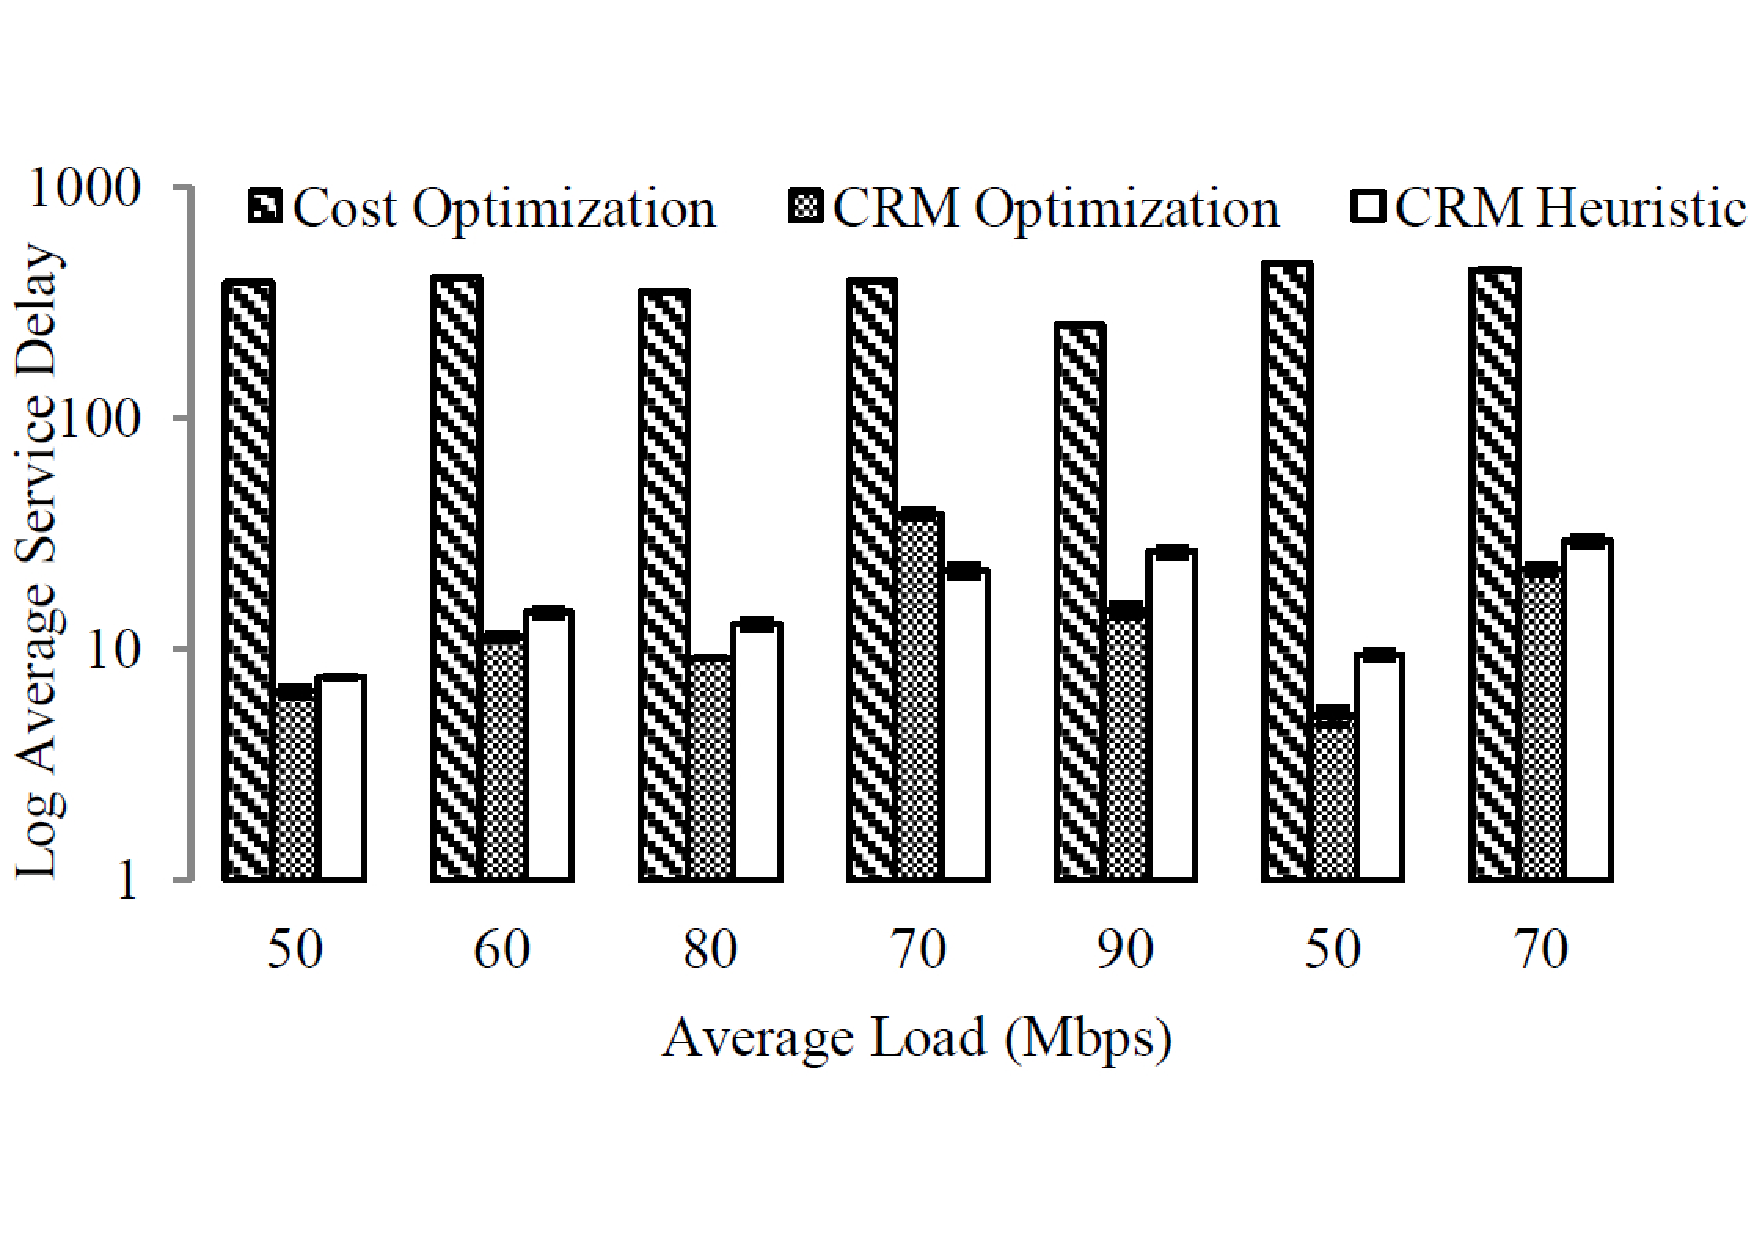
\includegraphics[trim=0 3cm 0 1cm,scale=0.25]{grafik/delay.pdf}
	\caption{Der heuristische Ansatz bewegt sich sehr nahe an der optimalen Verzögerung
	(Diagramm entnommen aus \cite{IEEEhowto:orig})}
	\label{img:delay}
\end{figure}

Der heuristische Ansatz ist dabei nur geringfügig im Nachteil gegenüber der Linearen Optimierung. Auch bei der Anzahl an Verschiebungen von Diensten zeigt sich ein ähnliches Bild. Wie in Abbildung \ref{img:VMMIG} zu sehen ist, sind die lineare Optimierung sowie die Heuristik deutlich besser als der naive Ansatz.

\begin{figure}[h!]
	\centering
	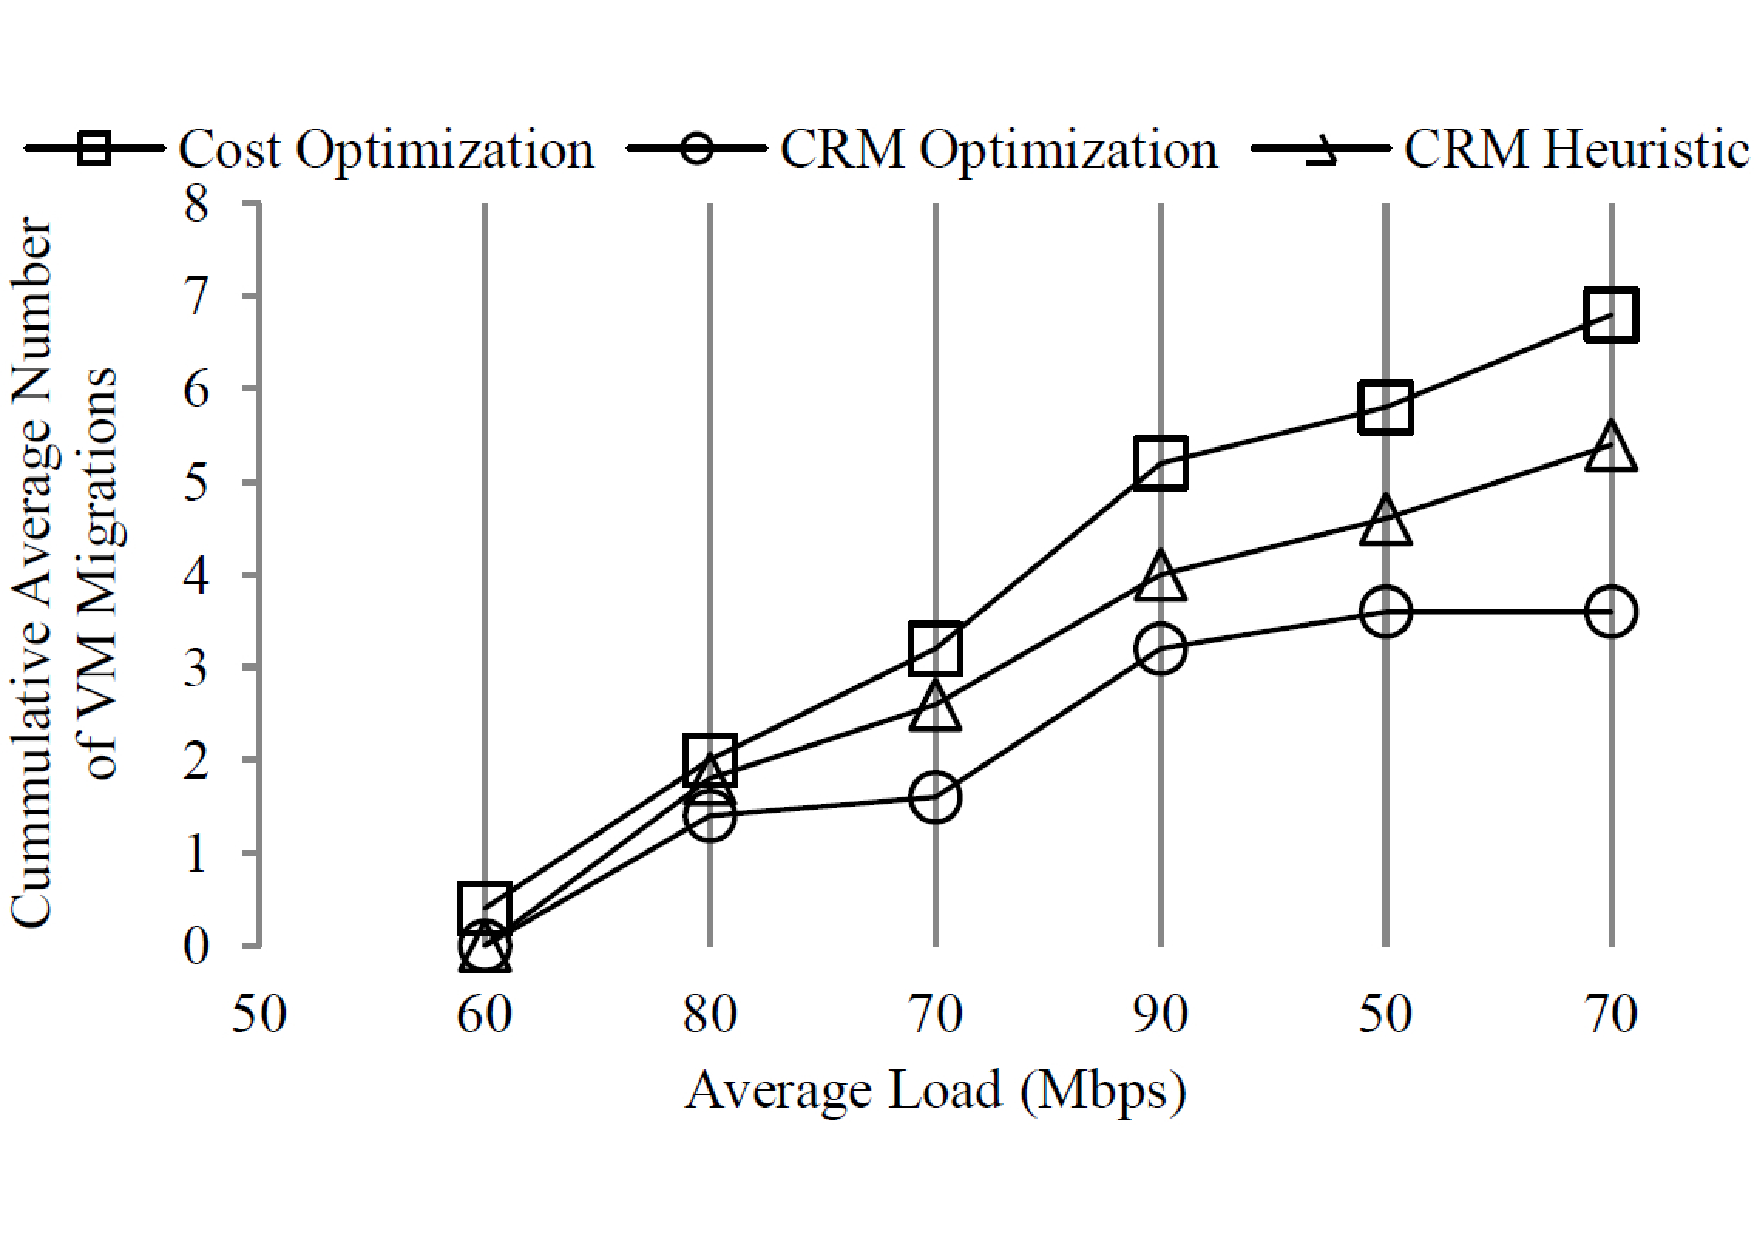
\includegraphics[trim=0 3cm 0 1cm,scale=0.25]{grafik/VMMIG.pdf}
	\caption{Die Heuristik schneidet besser ab als der naive Ansatz.
	(Diagramm entnommen aus \cite{IEEEhowto:orig})}
	\label{img:VMMIG}
\end{figure}

Was den Overhead in der Kontrollebene angeht, so performt hier die Heuristik am schlechtesten. 

\begin{figure}[h!]
	\centering
	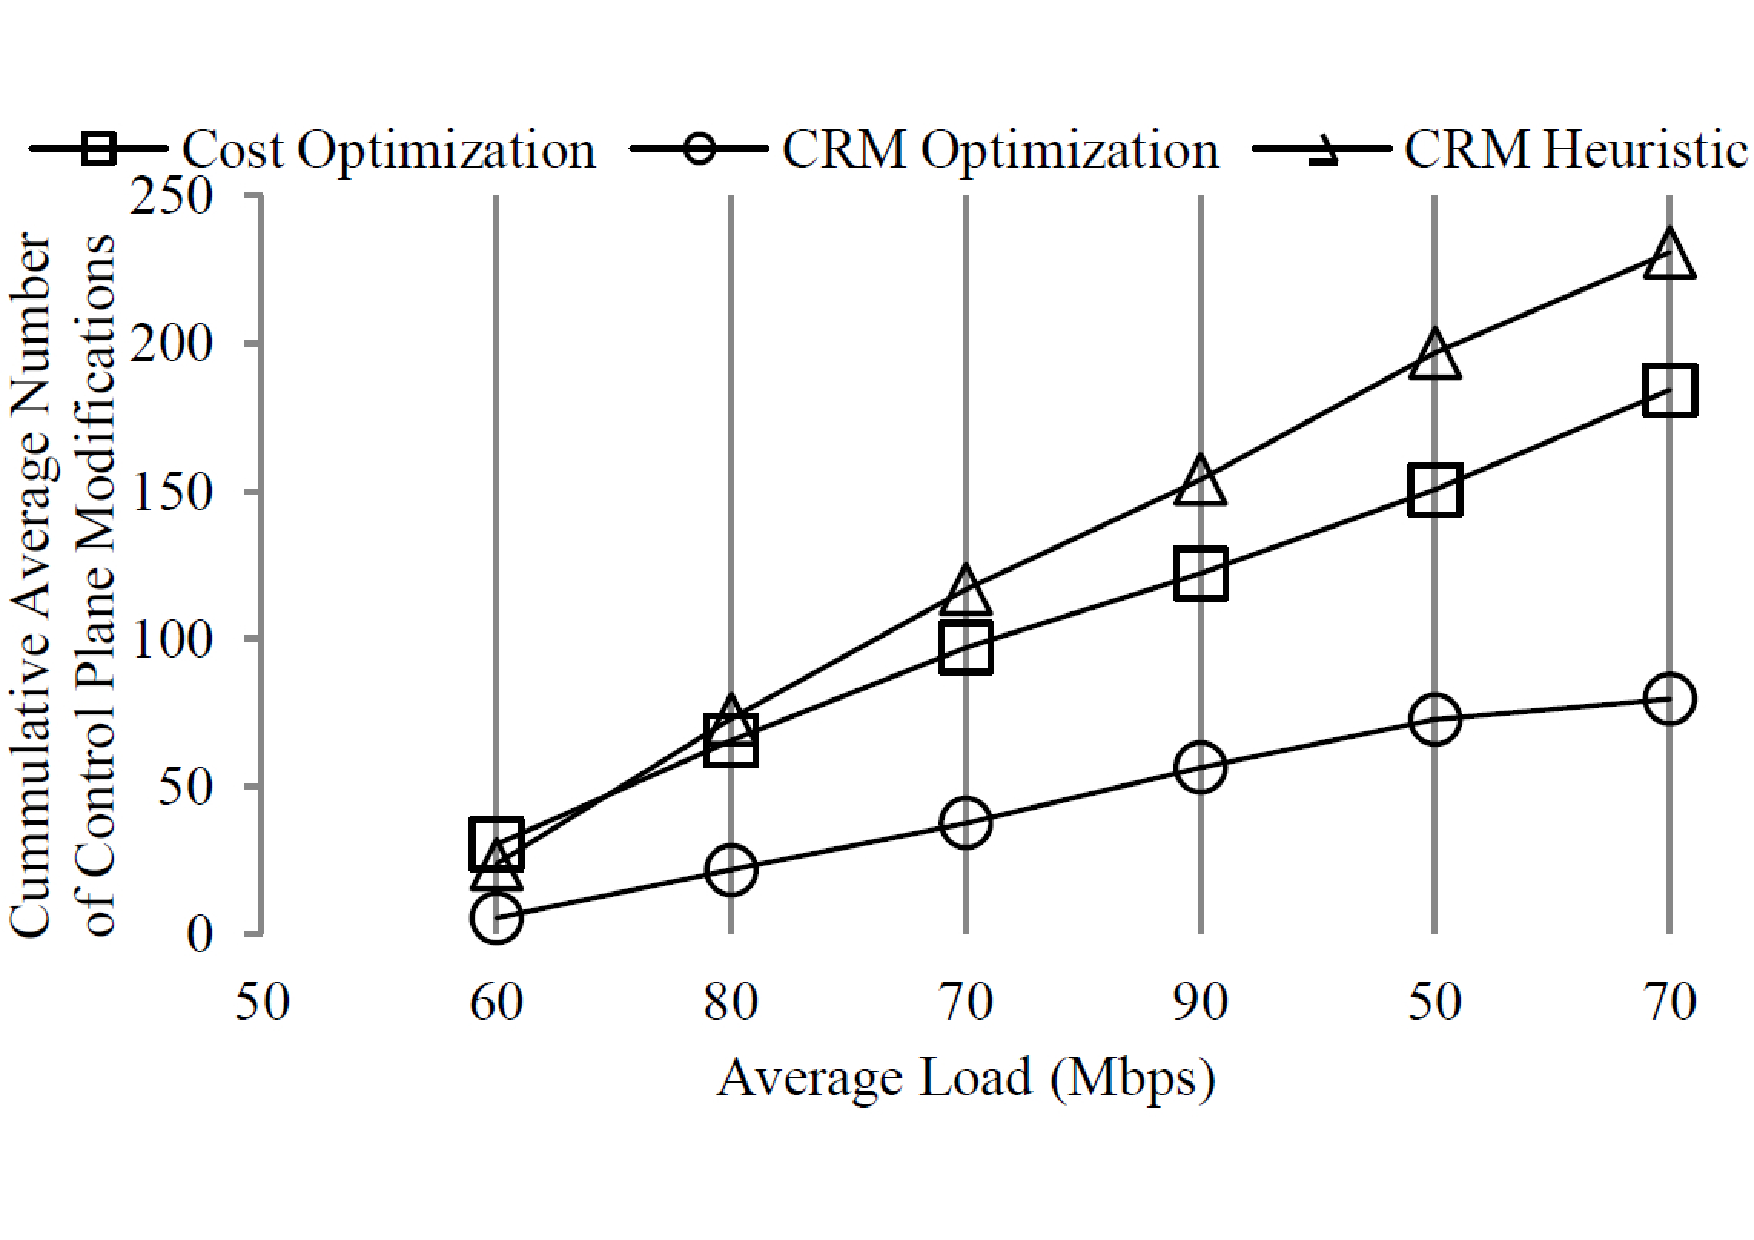
\includegraphics[trim=0 3cm 0 1cm,scale=0.25]{grafik/CPM.pdf}
	\caption{Die Heuristik verursacht am meisten Overhead in der Kontrollebene.
	(Diagramm entnommen aus \cite{IEEEhowto:orig})}
	\label{img:CPM}
\end{figure}


In Abbildung \ref{img:MDP} wird die Heuristik mit der Verbesserung durch den MDP mit der Heuristik ohne diese Verbesserung verglichen. Man sieht, dass die Verbesserung durch den MDP  anfänglich mehr VM Verschiebungen verursacht. Dies erweist sich aber als vorteilhaft, indem es auf lange Sicht insgesamt zu weniger Verschiebungen kommt.

\begin{figure}[h!]
	\centering
	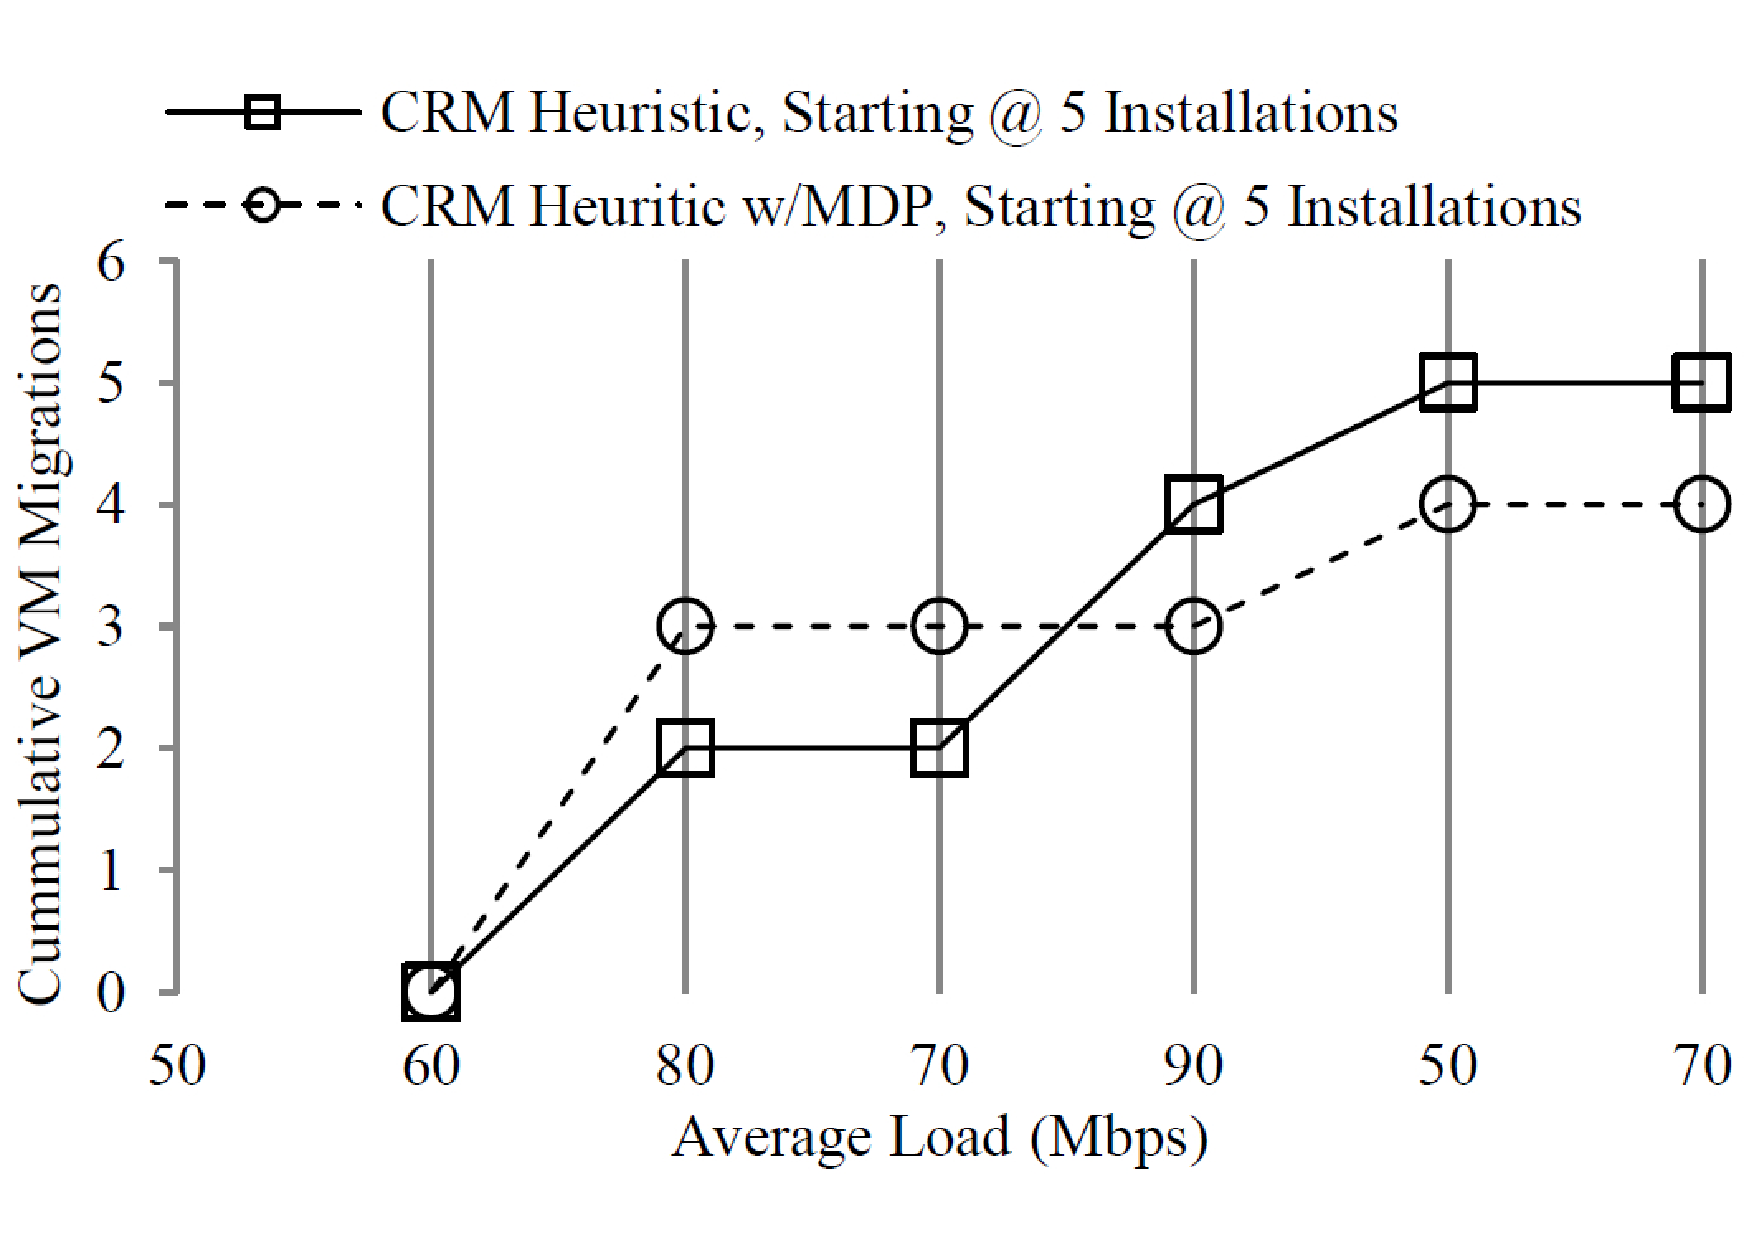
\includegraphics[trim=0 2cm 0 1cm,scale=0.25]{grafik/MDP.pdf}
	\caption{Über einen langen Zeitraum ist machen sich die Vorteile des MDP bemerkbar.
	(Diagramm entnommen aus \cite{IEEEhowto:orig})}
	\label{img:MDP}
\end{figure}



\section{Fazit}

In diesem Paper wurde in Form einer Zusammenfassung eine neuartige RSU Cloud mit zugehörigem Ressourcen Management vorgestellt. Der große Vorteil dieser Architektur ist, dass sie dank SDN flexibel konfigurierbar ist und sich somit dynamisch an die Nachfrage anpassen lässt. Dies spart Kosten für den Dienstanbieter und wirkt sich zudem positiv auf die Latenzzeiten aus, da die Dienste möglichst nah am Konsumenten gehostet werden. Ein weiterer Vorteil ist, dass sich die Architektur leicht neben schon bestehenden, anderen Cloud Architekturen einsetzen lässt.
Außerdem wurde eine Lösung für das Ressourcen Management in der Cloud gefunden, die gleichzeitig die Verschiebung von VMs, den Overhead in der Kontrollebene, die Anzahl an Hosts im Netz sowie die Verzögerung optimiert.
Eine Einführung in SDN sowie die Betrachtung anderer Cloud Architekturen geben nützliche Hintergrundinformationen zum Themengebiet.


% trigger a \newpage just before the given reference
% number - used to balance the columns on the last page
% adjust value as needed - may need to be readjusted if
% the document is modified later
%\IEEEtriggeratref{8}
% The "triggered" command can be changed if desired:
%\IEEEtriggercmd{\enlargethispage{-5in}}

% references section

% can use a bibliography generated by BibTeX as a .bbl file
% BibTeX documentation can be easily obtained at:
% http://www.ctan.org/tex-archive/biblio/bibtex/contrib/doc/
% The IEEEtran BibTeX style support page is at:
% http://www.michaelshell.org/tex/ieeetran/bibtex/
%\bibliographystyle{IEEEtran}
% argument is your BibTeX string definitions and bibliography database(s)
%\bibliography{IEEEabrv,IEEEexample}
%
% <OR> manually copy in the resultant .bbl file
% set second argument of \begin to the number of references
% (used to reserve space for the reference number labels box)

\newpage

\begin{thebibliography}{1}

\bibitem{IEEEhowto:orig}
Mohammad A. Salahuddin, Ala Al-Fuqaha, Mohsen Guizani \emph{Software Defined Networking for RSU Clouds in support of The Internet of Vehicles}, IEEE Internet of Things Journal, VOL. X, NO. X, November 2014.


\bibitem{IEEEhowto:sdn}
Michael Jarschel, Thomas Zinner, Tobias Hoßfeld, Phuoc Tran-Gia, and Wolfgang Kellerer \emph{Interfaces, attributes, and use cases: A compass for SDN}, Communications Magazine, IEEE, 2014.


\bibitem{IEEEhowto:star}
K. Mershad and H. Artail \emph{Finding a STAR in a Vehicular Cloud}, IEEE
Intelligent Transportation Systems Magazine, vol. 5, no. 2, pp. 55-68, 2013.

\bibitem{IEEEhowto:rethinking}
R. Hussain, J. Son, H. Eun, S. Kim and H. Oh \emph{Rethinking Vehicular
Communications: Merging VANET with cloud computing}, IEEE 4th
International Conference on Cloud Computing Technology and Science
(CloudCom), Taipei, 2012.

\bibitem{IEEEhowto:king}
G. Curry and R. Feldman \emph{Manufacturing Systems Modeling and Analysis}, Springer Heidelberg Dordrecht, 2nd Edition, 2011.

\bibitem{IEEEhowto:sum}
Mohammad A. Salahuddin, Ala Al-Fuqaha, Mohsen Guizani and Soumaya Cherkaoui \emph{RSU Cloud and its Resource Management in
support of Enhanced Vehicular Applications}, Globecom 2014 Workshop - Cloud Computing Systems, Networks, and Applications, 2014.








\end{thebibliography}

\end{document}


